\chapter{Графический материал}\label{appendix-diagrams}							% Заголовок

\section{Диаграмма классов UML}
\begin{figure}[ht] 
	\center
	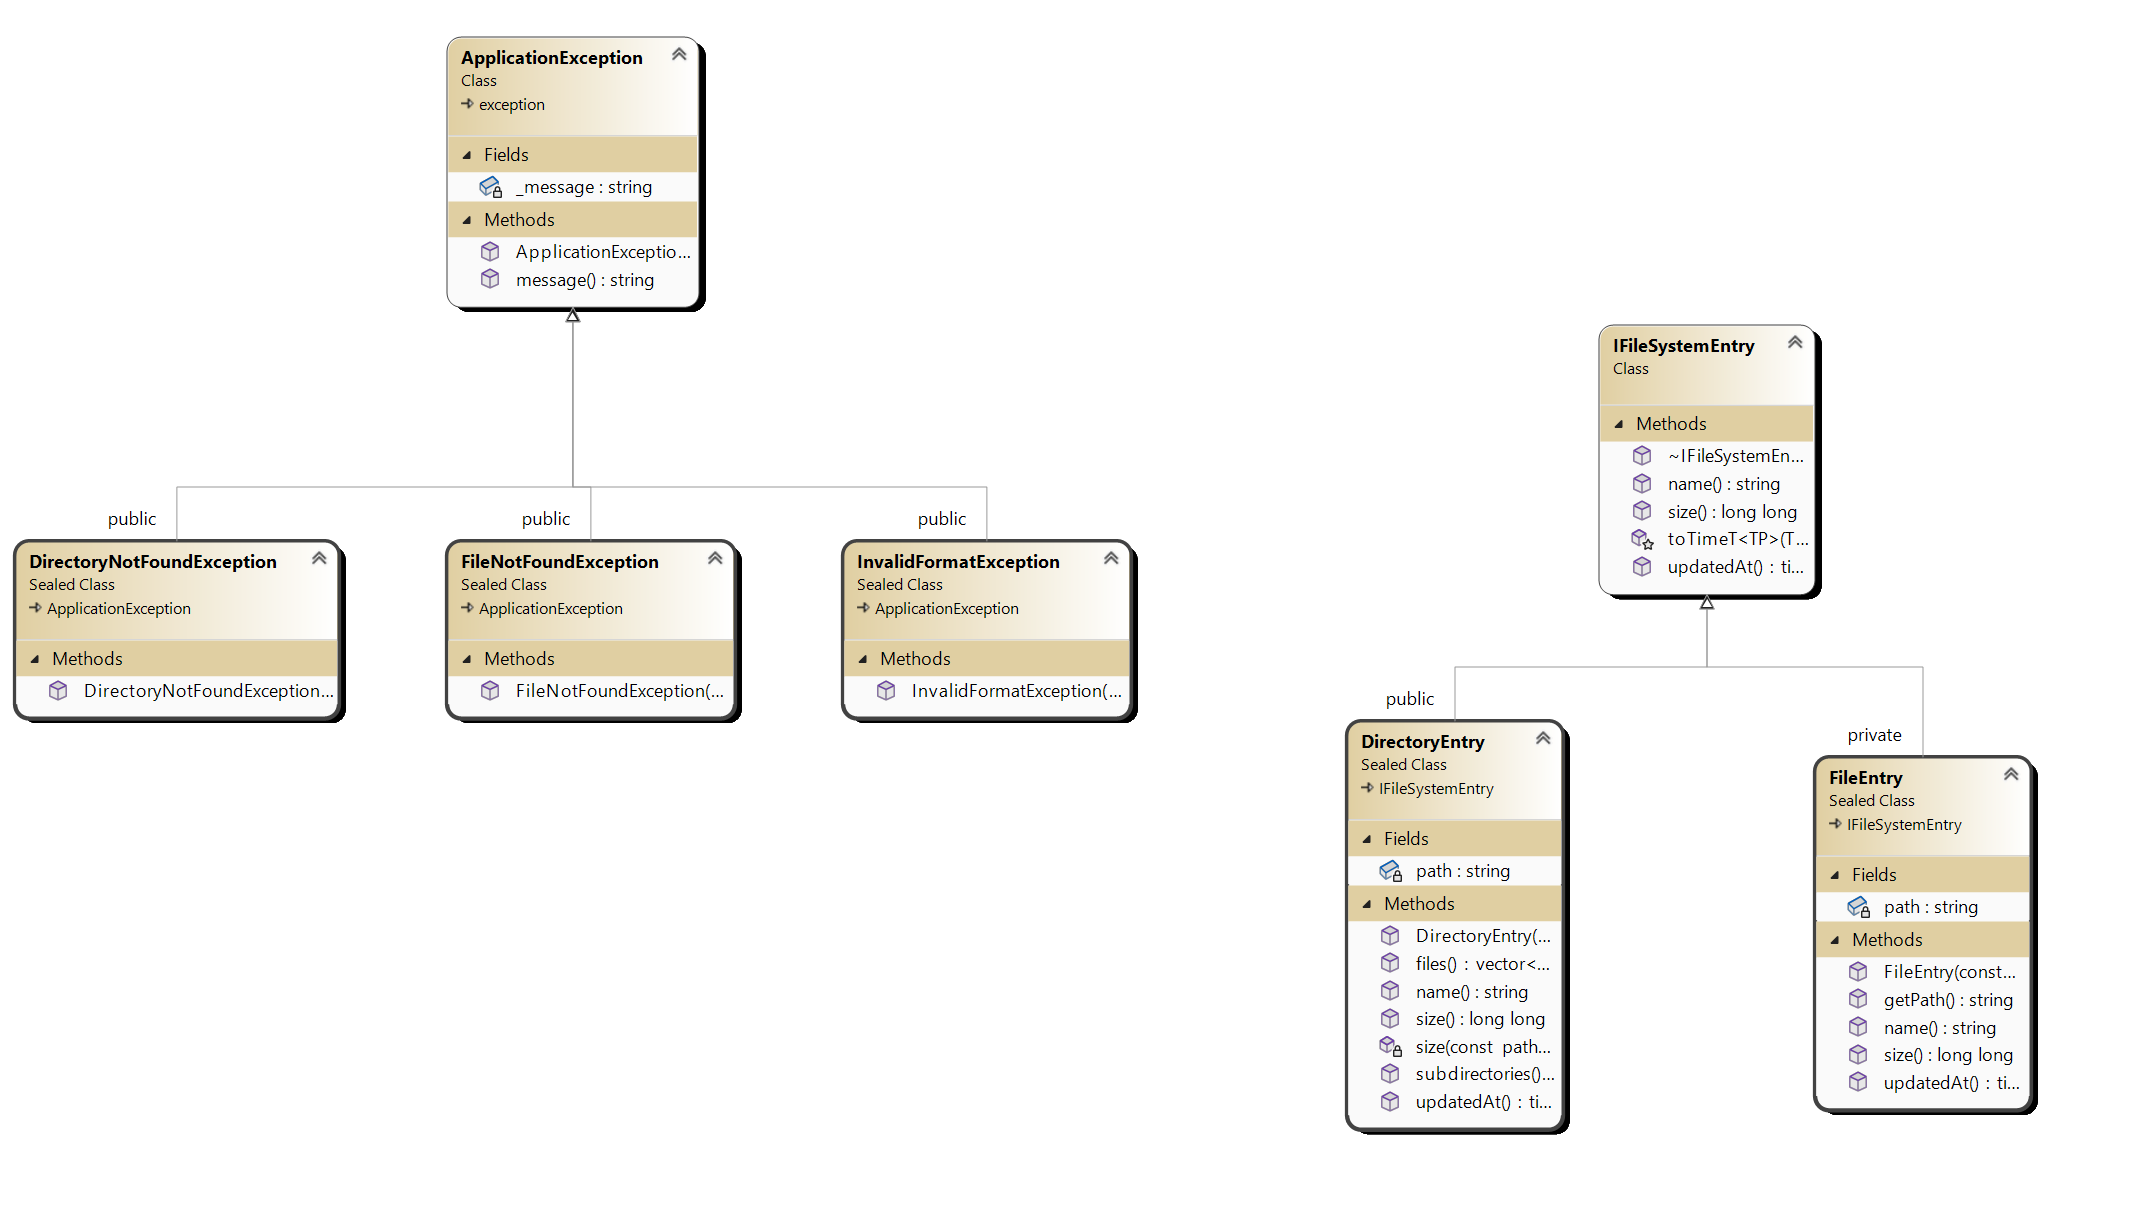
\includegraphics [scale=0.4] {my_folder/images/uml2.png}
	\caption{диаграмма классов UML 1} 
	\label{fig:uml1}  
\end{figure}\newpage
\begin{figure}[ht] 
	\center
	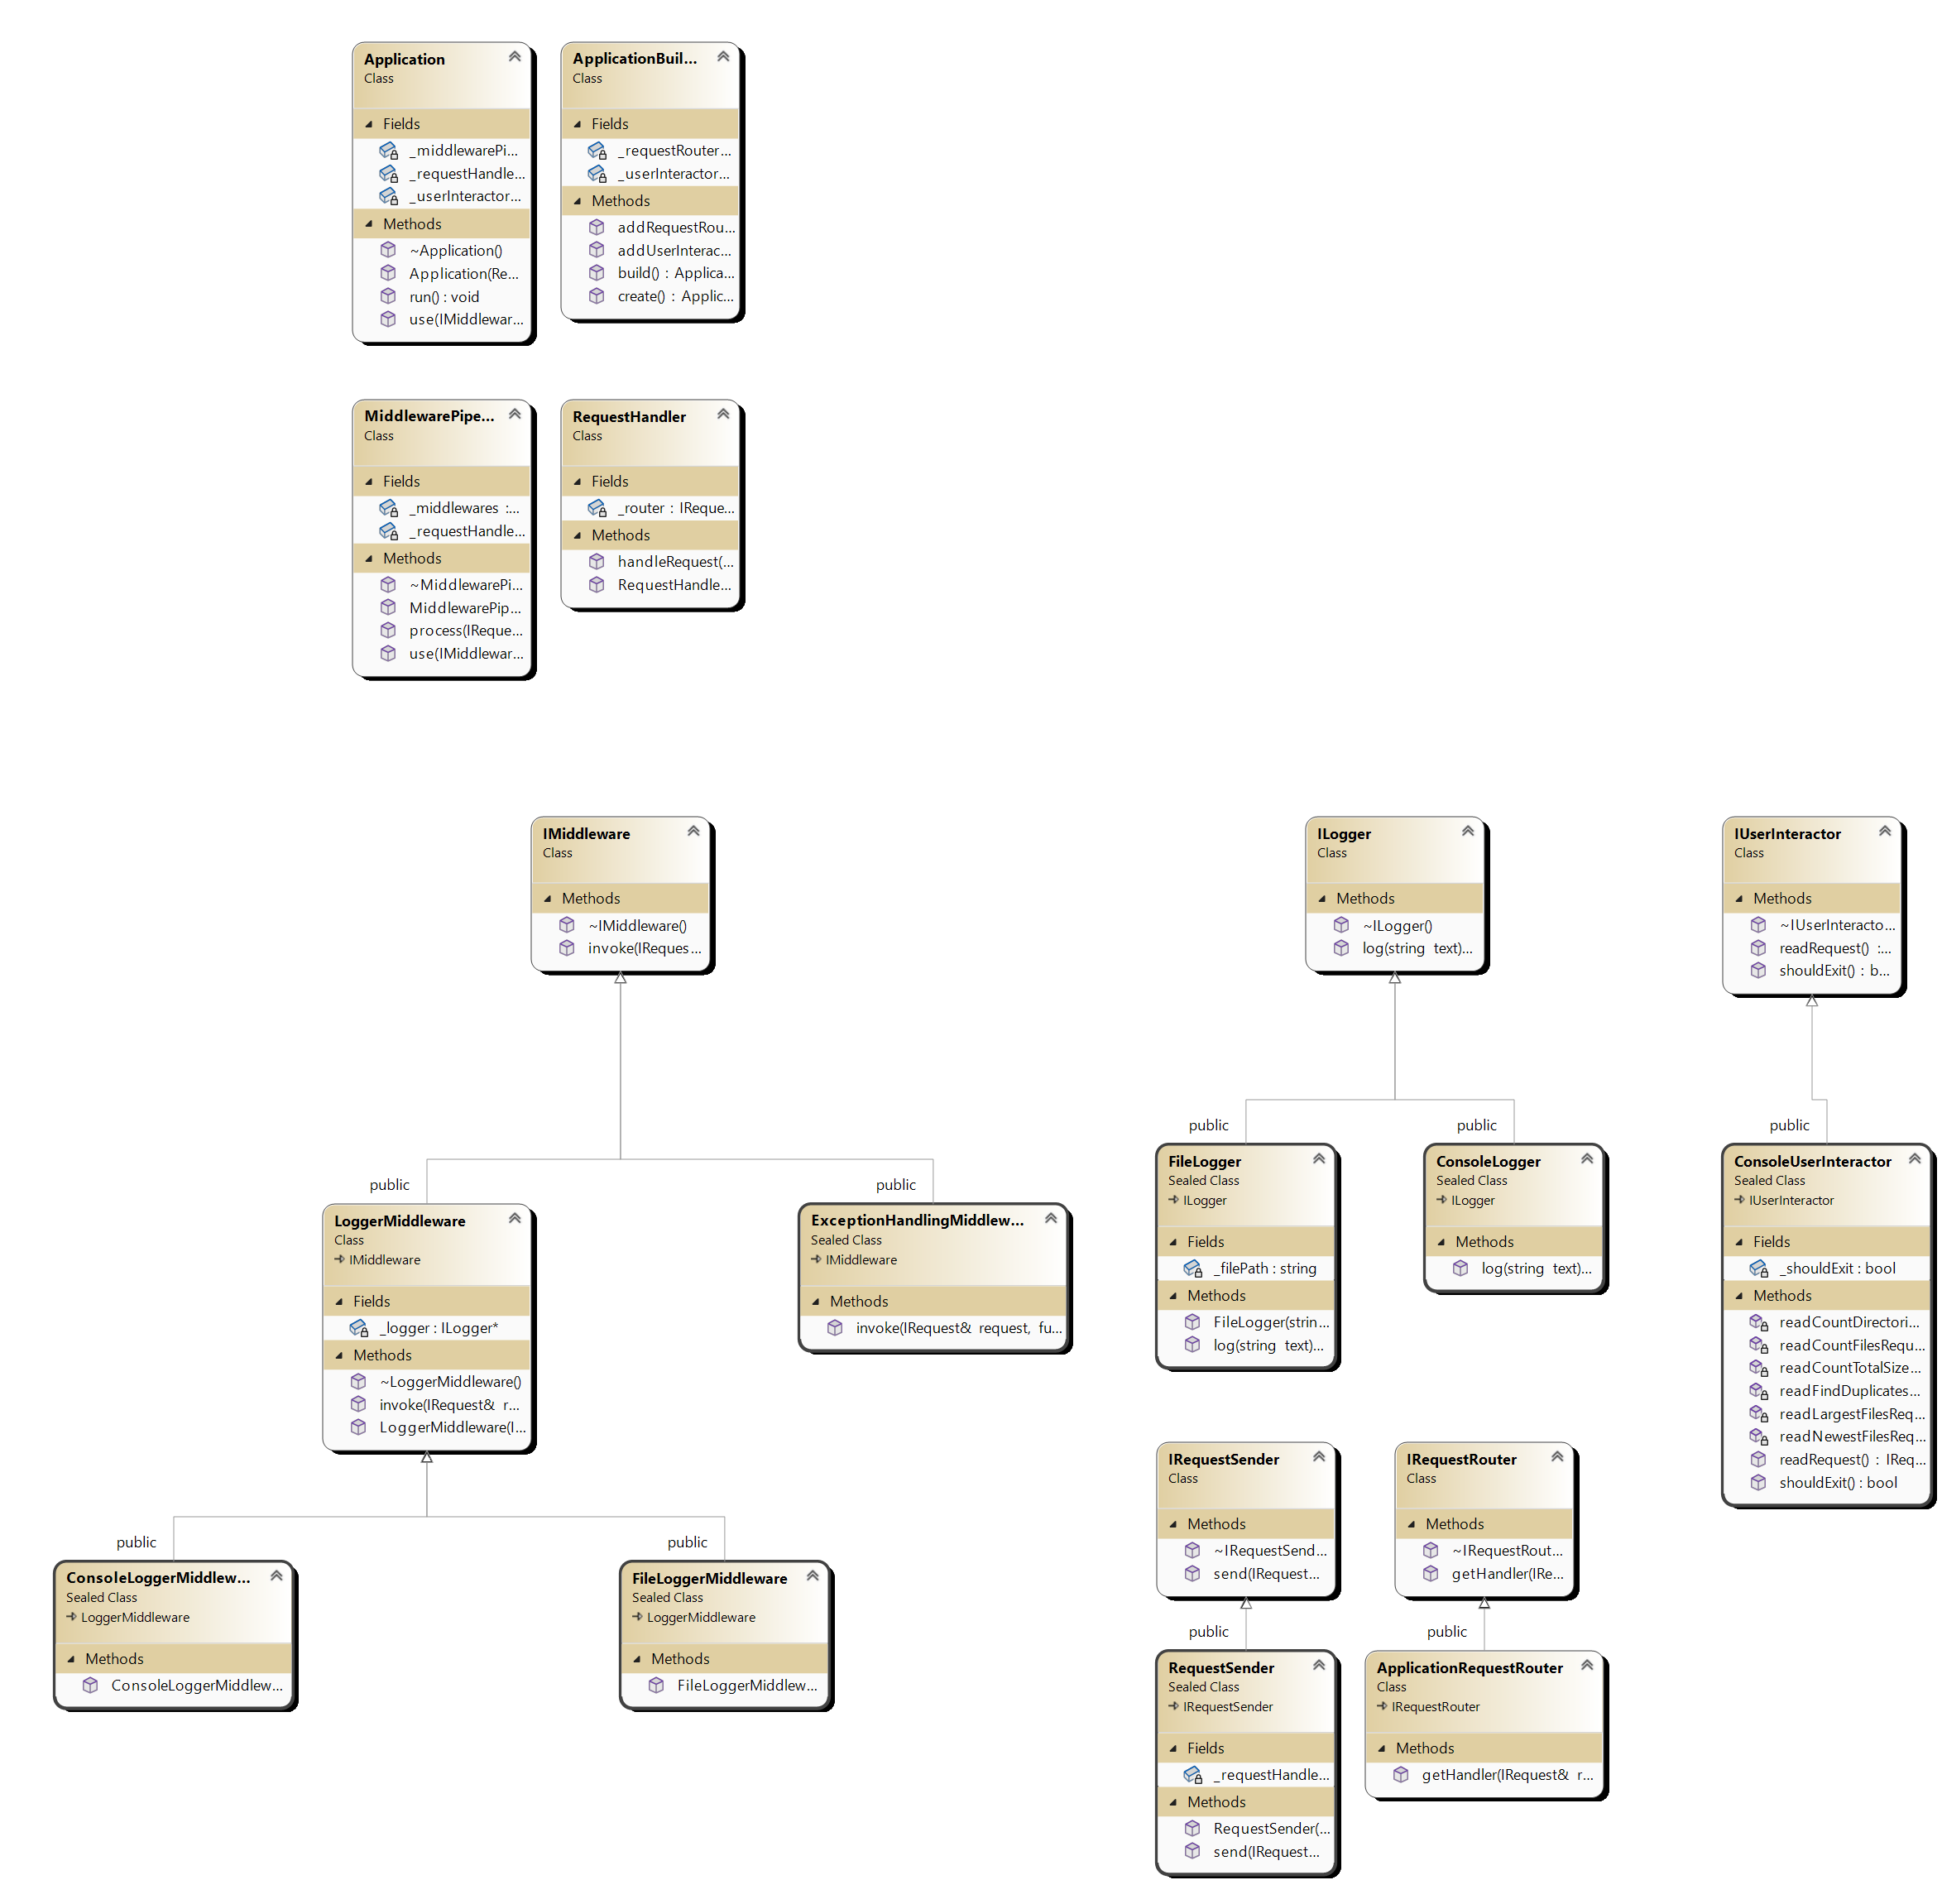
\includegraphics [scale=0.34] {my_folder/images/uml4.png}
	\caption{диаграмма классов UML 2} 
	\label{fig:uml2}  
\end{figure}\newpage
\begin{figure}[ht] 
	\center
	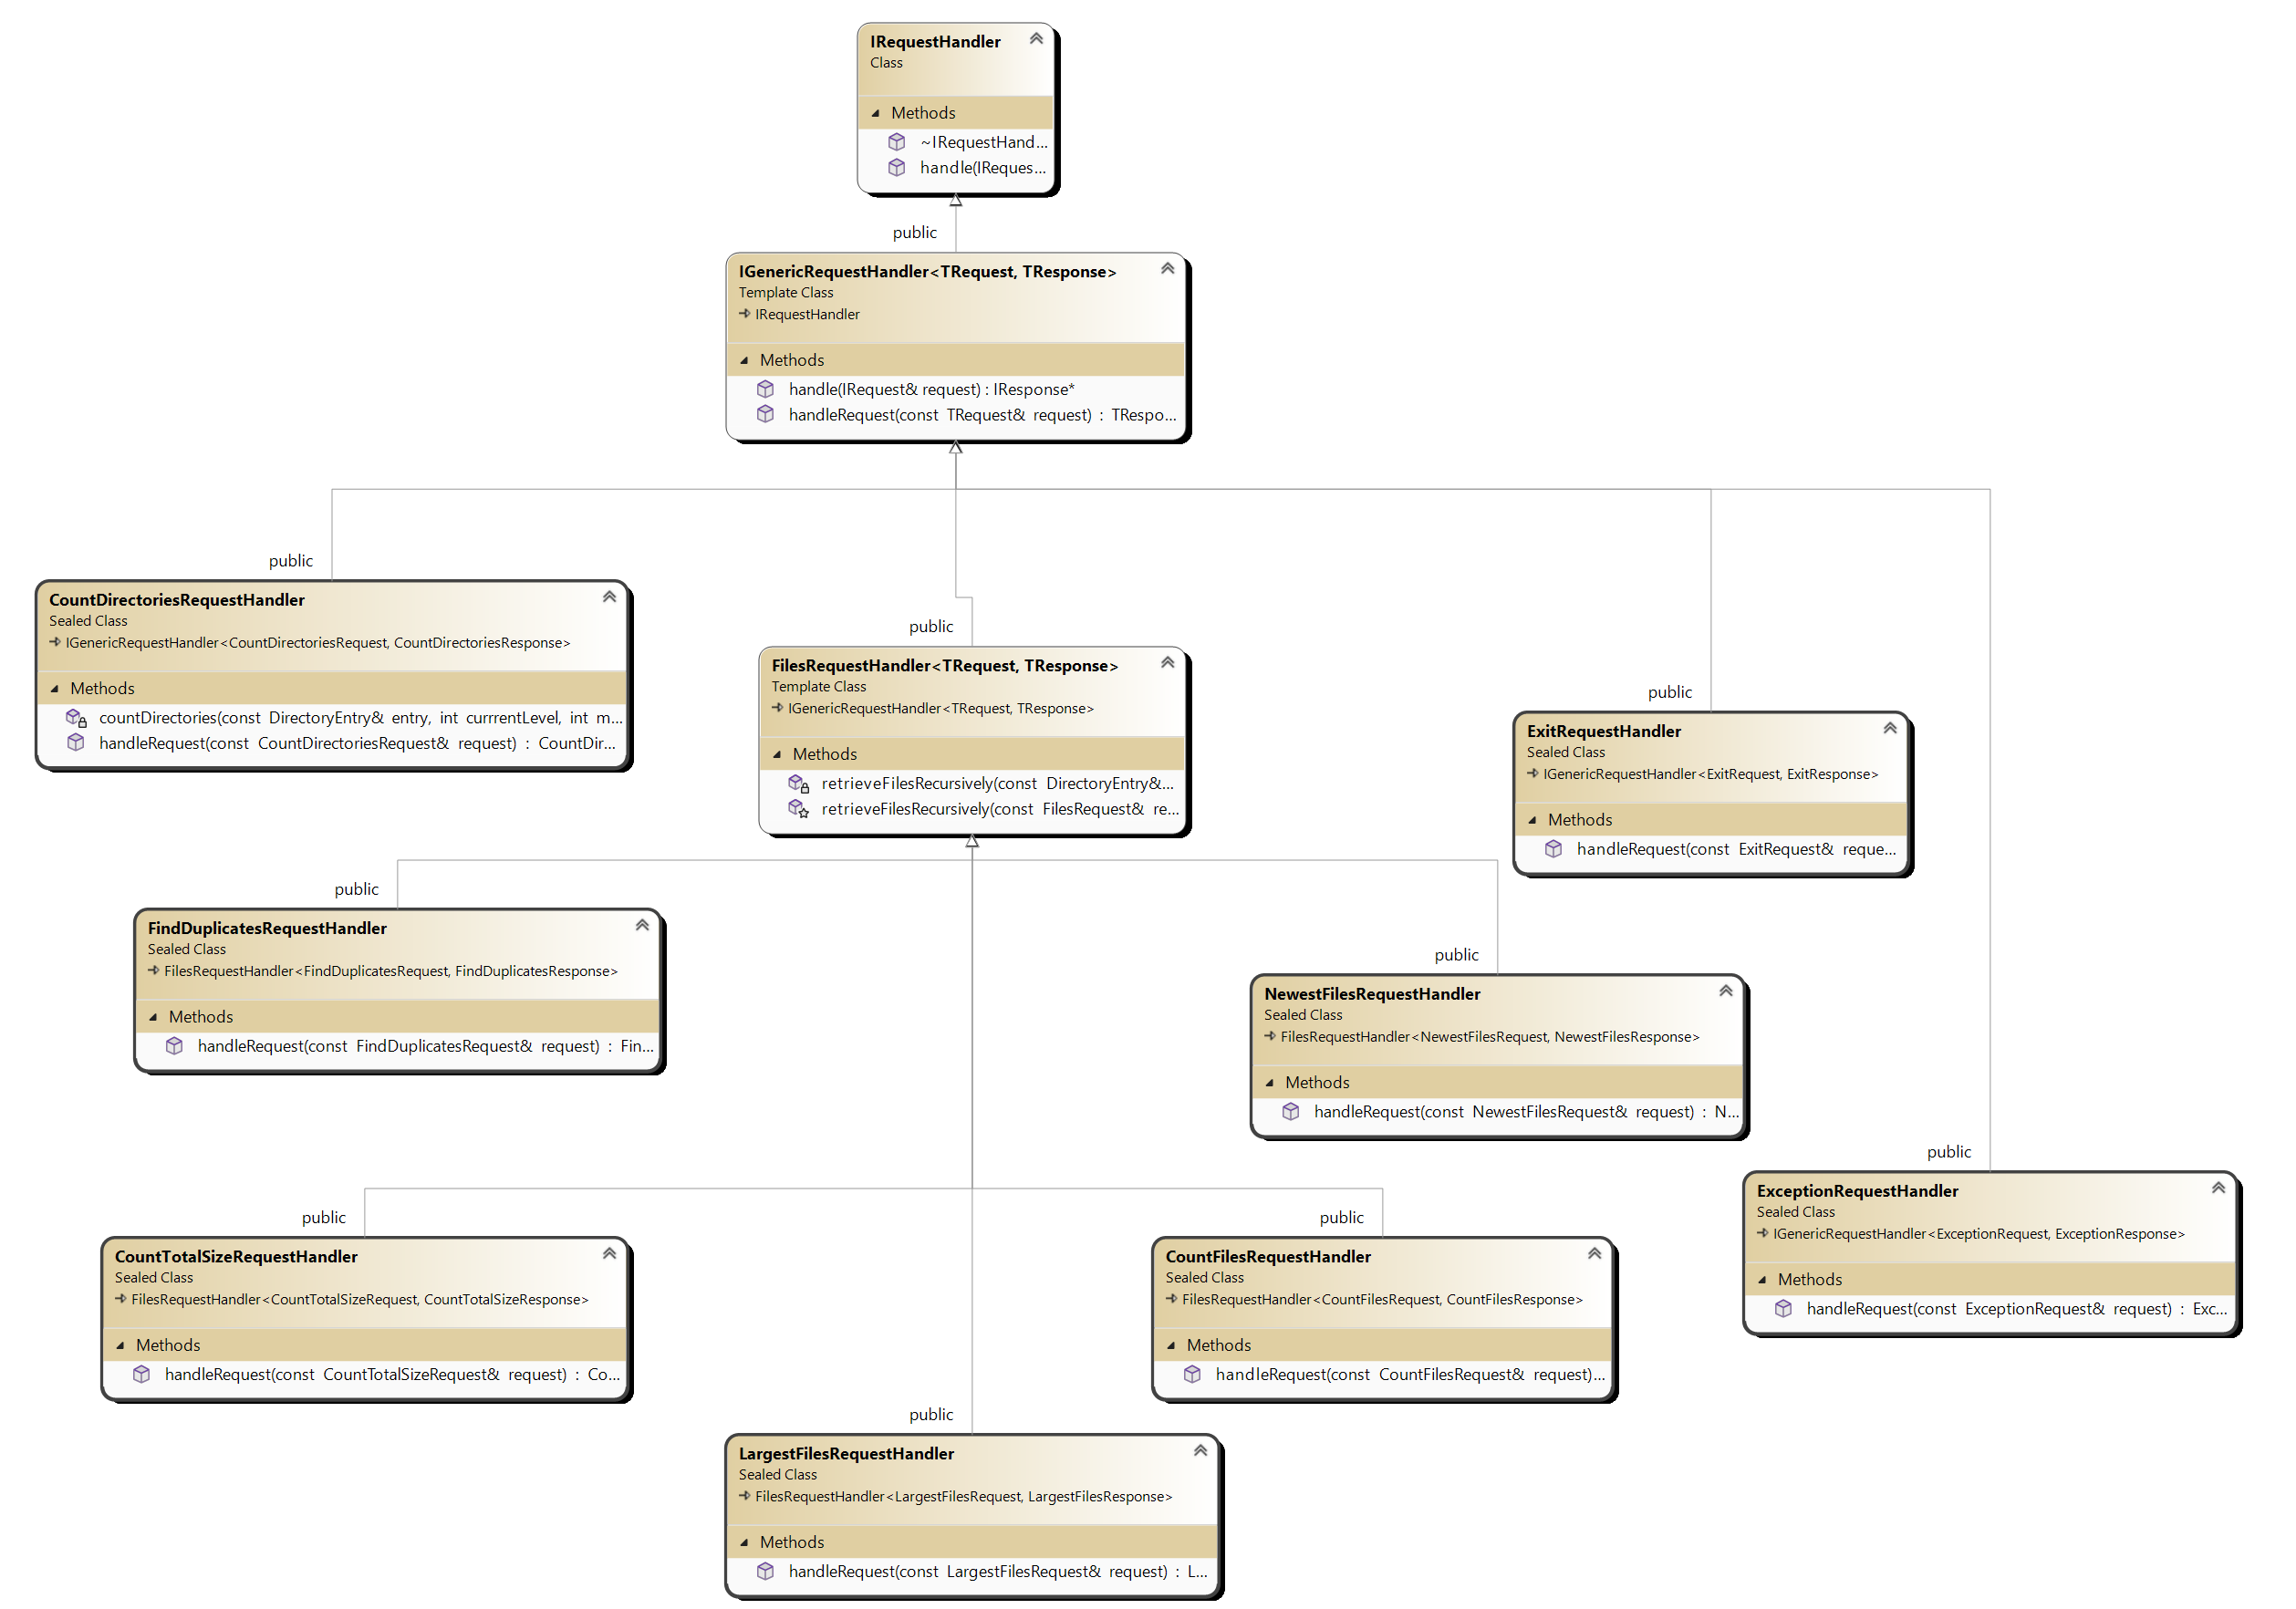
\includegraphics [scale=0.35] {my_folder/images/uml5.png}
	\caption{диаграмма классов UML 3} 
	\label{fig:uml3}  
\end{figure}\newpage
\begin{figure}[ht] 
	\center
	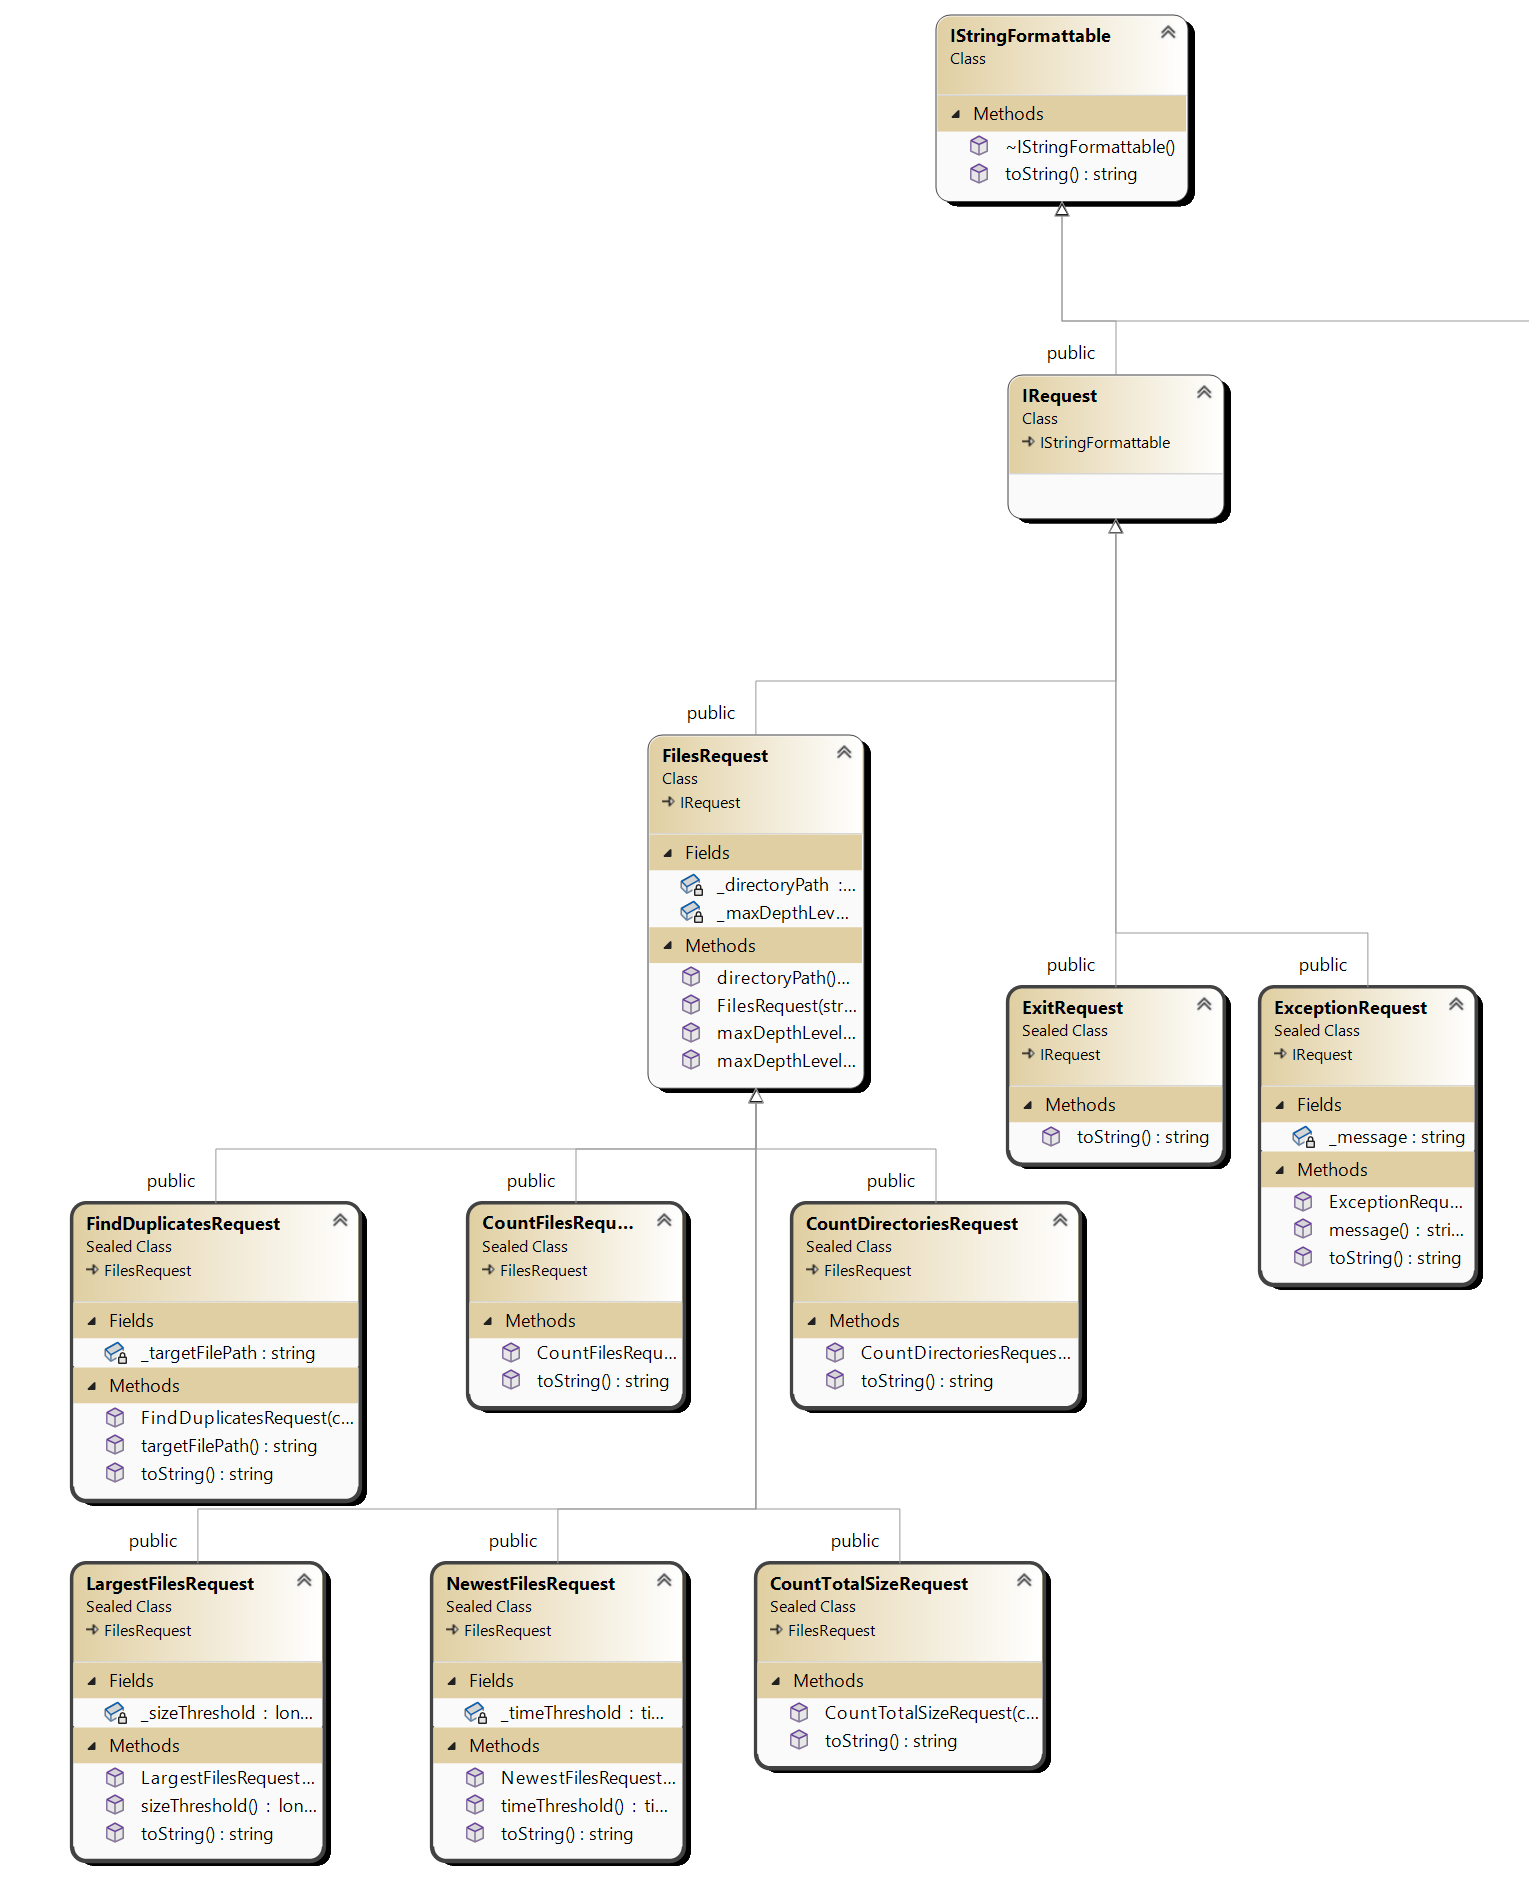
\includegraphics [scale=0.4] {my_folder/images/uml6.png}
	\caption{диаграмма классов UML 4} 
	\label{fig:uml4}  
\end{figure}\newpage
\begin{figure}[ht] 
	\center
	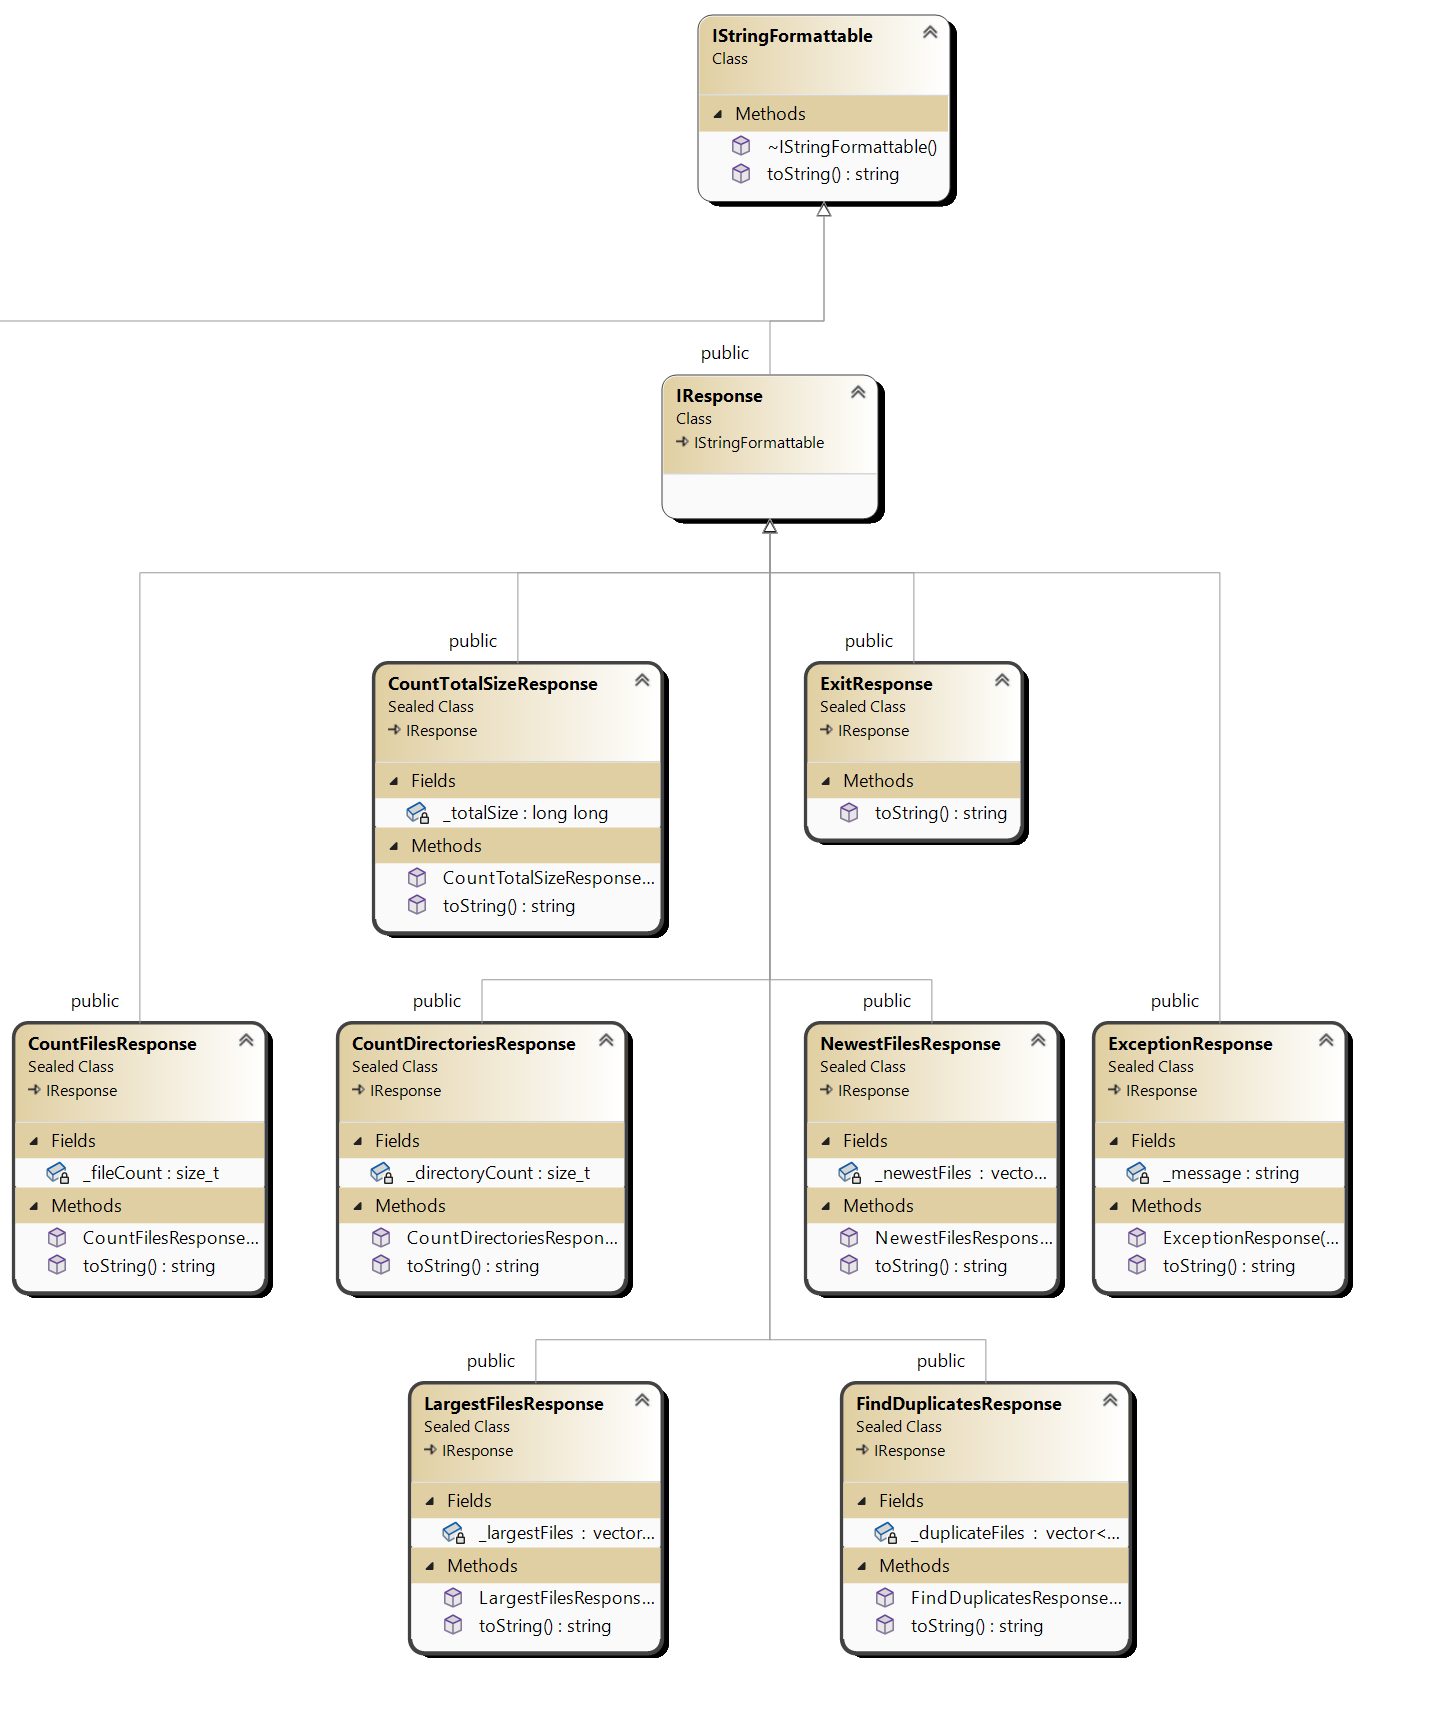
\includegraphics [scale=0.6] {my_folder/images/uml7.png}
	\caption{диаграмма классов UML 5} 
	\label{fig:uml5}  
\end{figure}\newpage

\section{Диаграммы IDEF0}
\begin{figure}[ht] 
	\center
	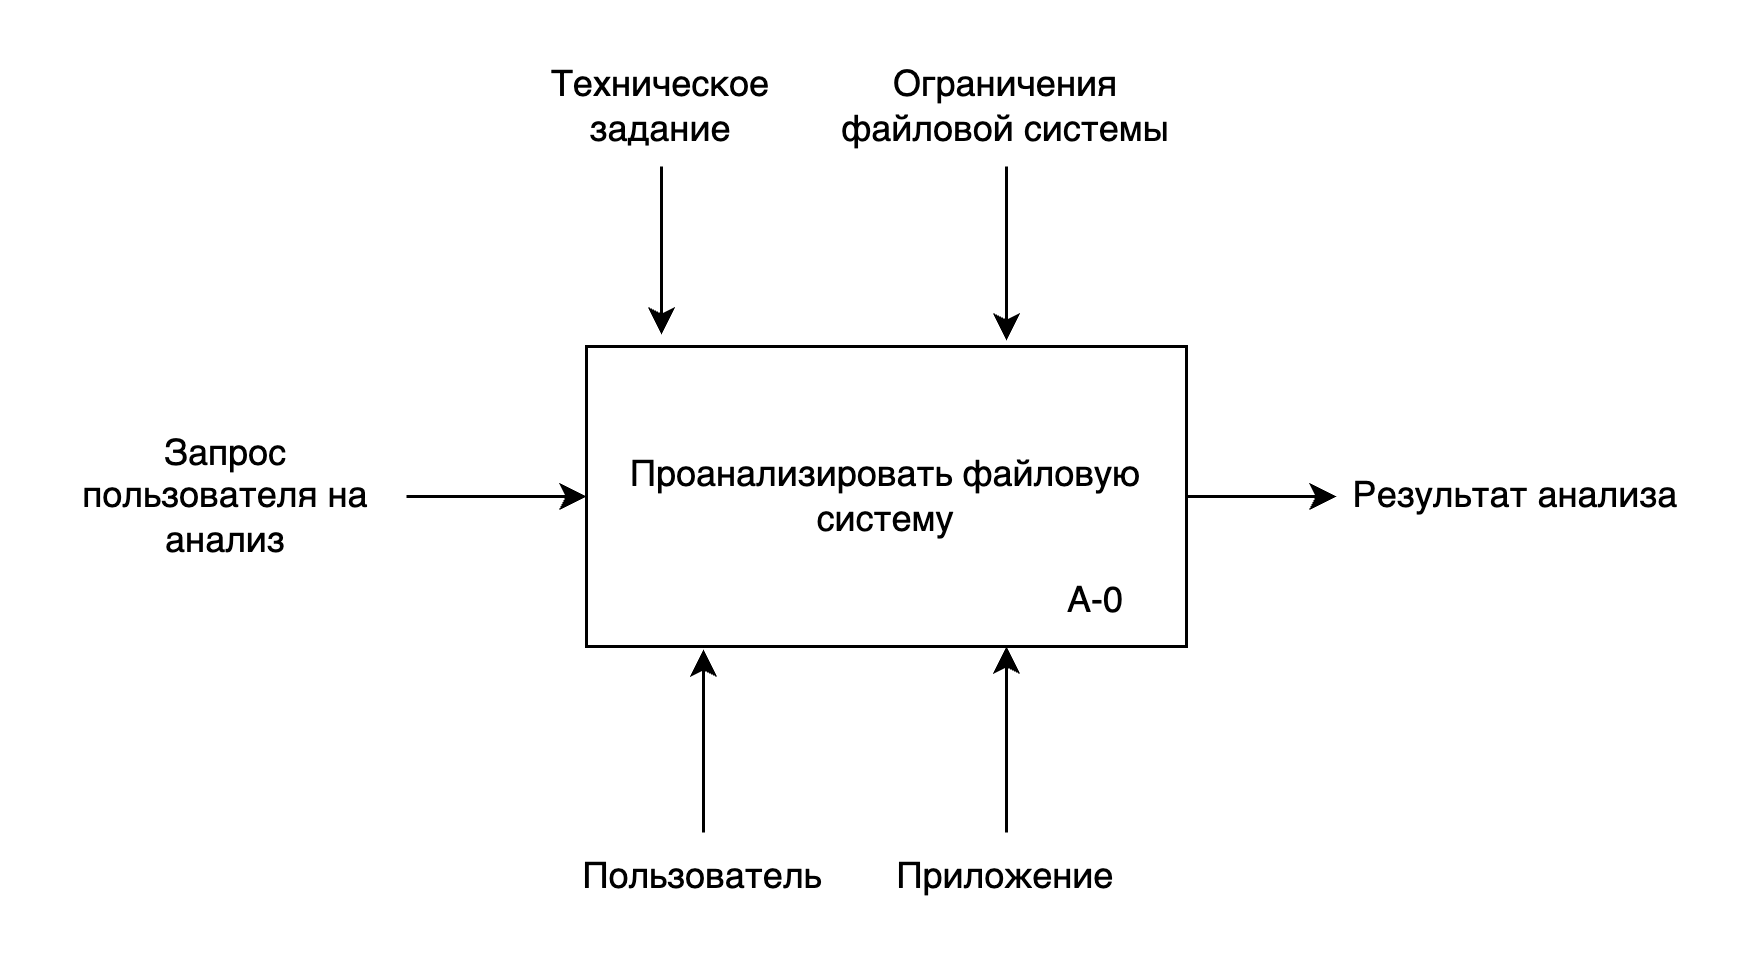
\includegraphics [scale=0.2] {my_folder/images/IDEF.png}
	\caption{диаграмма IDEF0 A-0} 
	\label{fig:idef0-A-0-a}  
\end{figure}
\begin{figure}[ht] 
	\center
	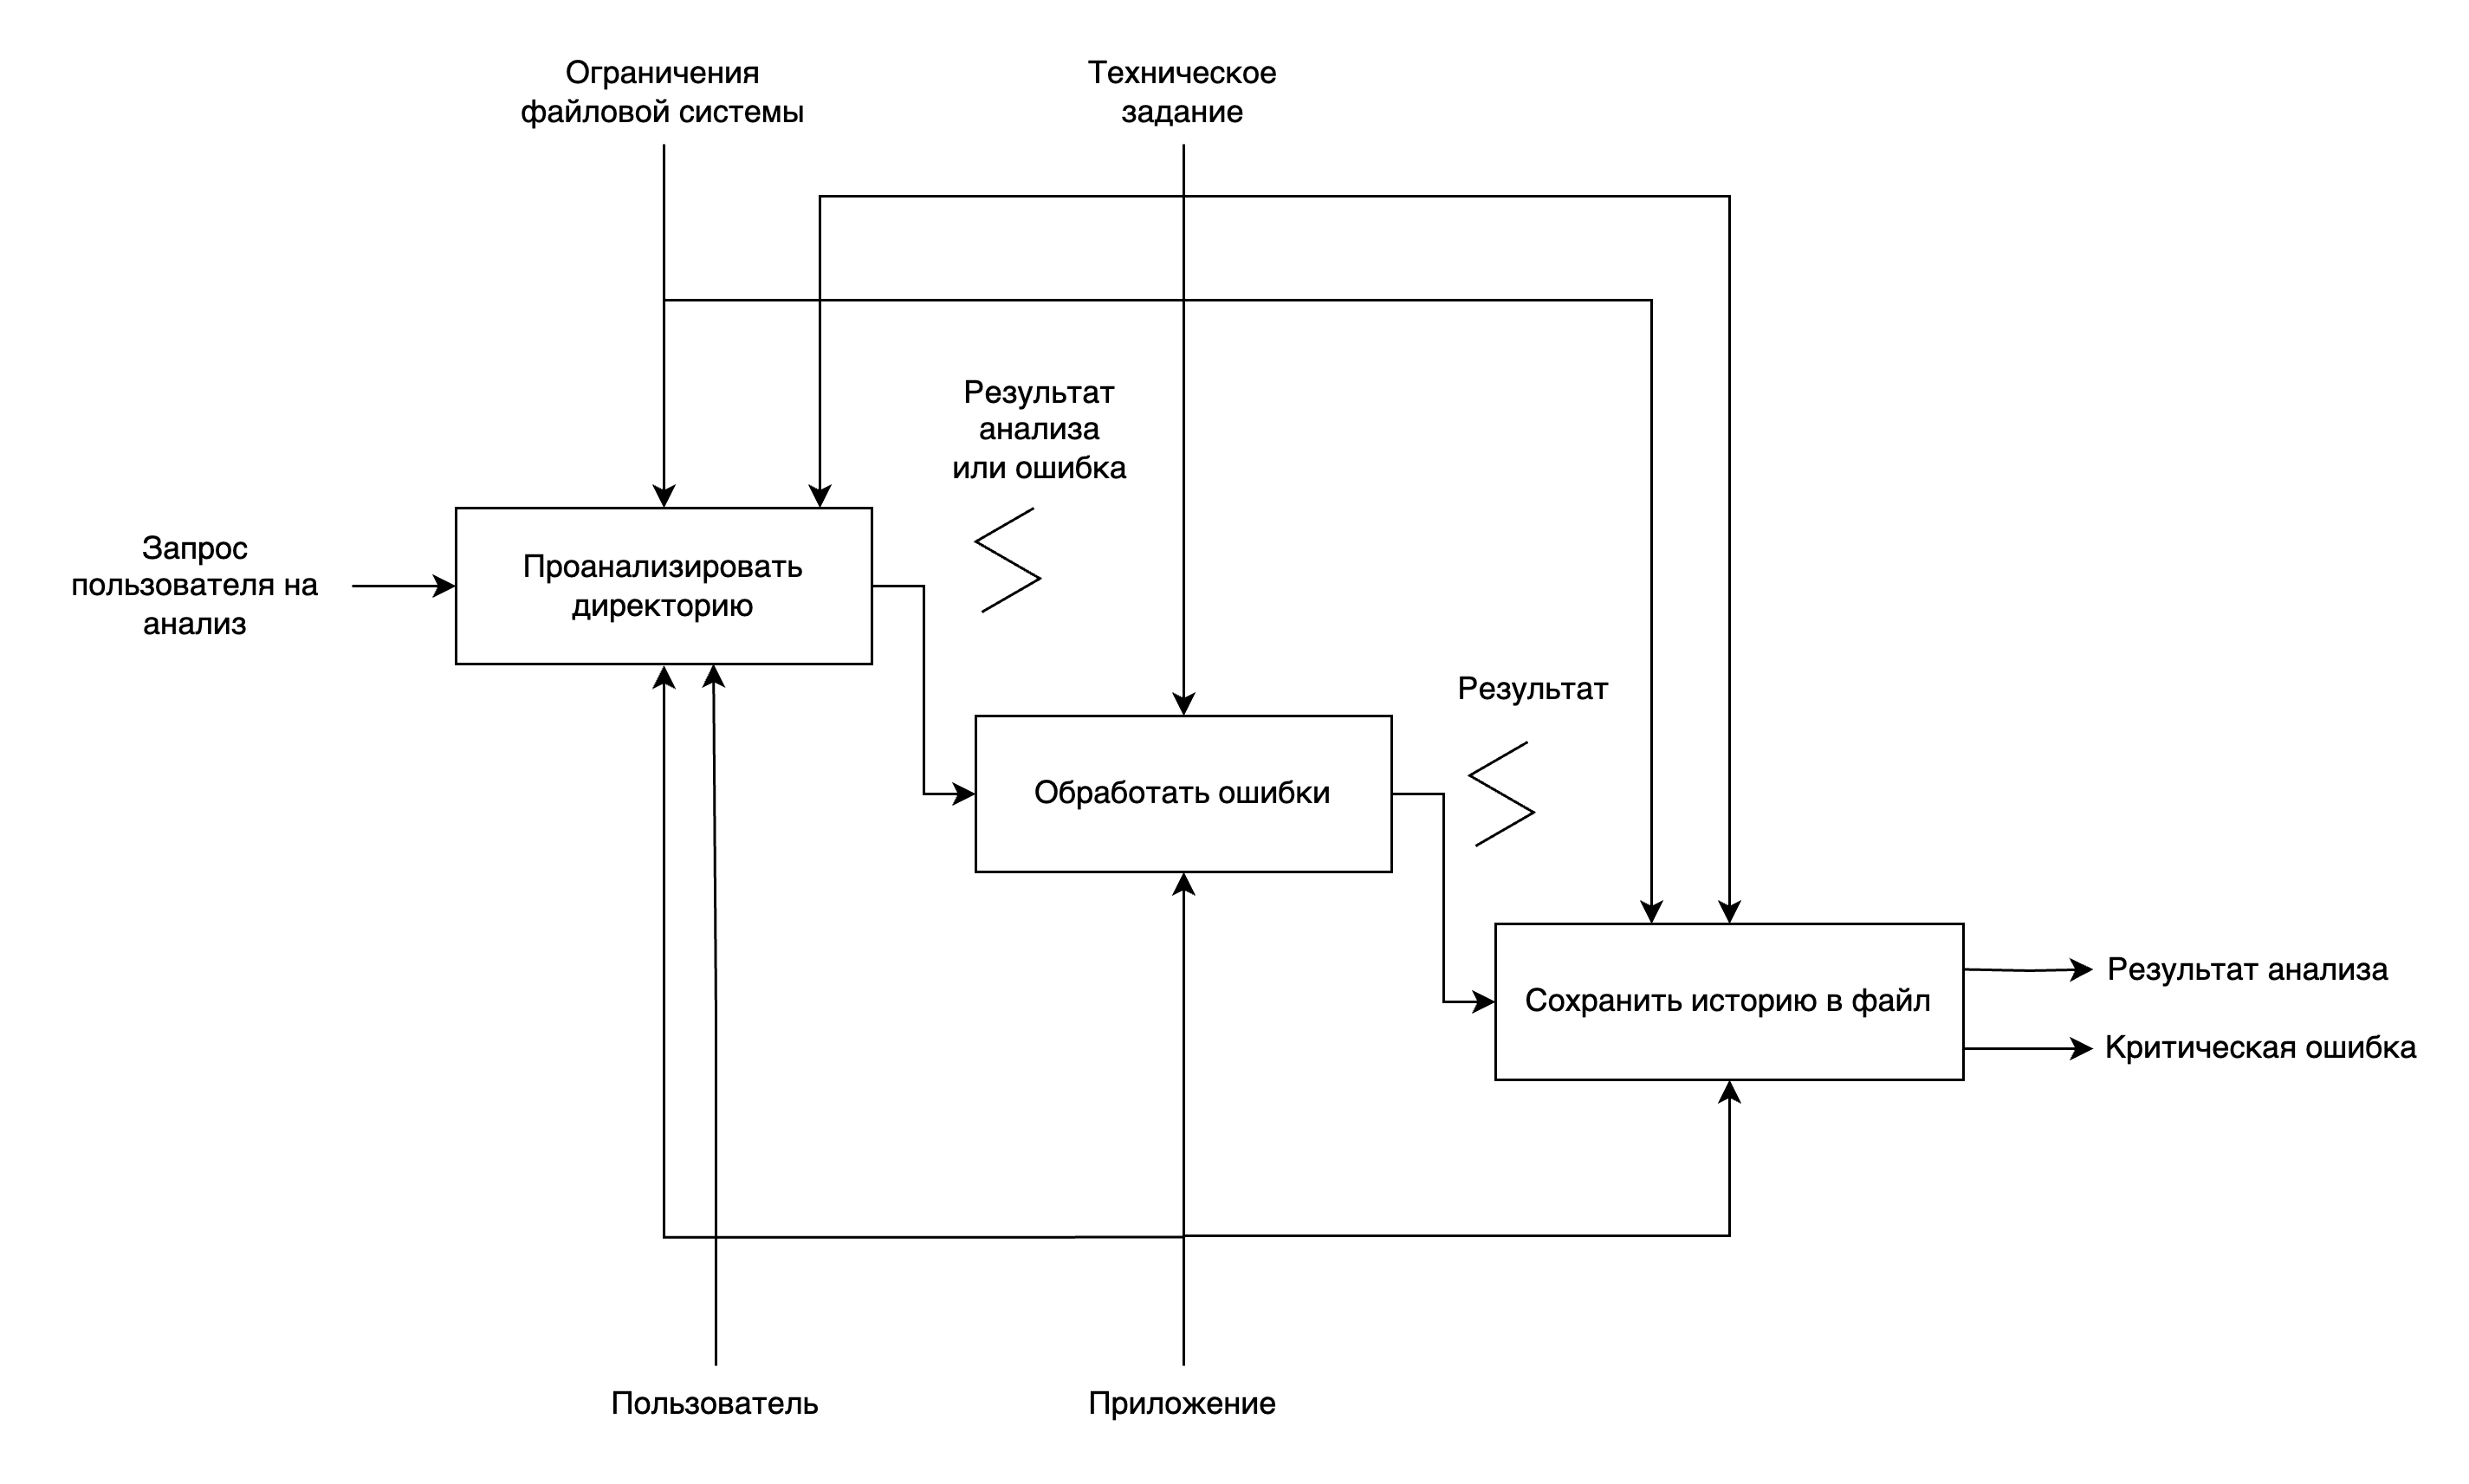
\includegraphics [scale=0.15] {my_folder/images/IDEF0_A0.png}
	\caption{диаграмма IDEF0 A0} 
	\label{fig:idef0-A0-a}  
\end{figure}


%% В случае, когда таблица (рисунок) размещаются на последней странице, для переноса названия приложения на новую строку используем:
% \NewPage % начать новое приложение с новой страницы 